\documentclass[a4j,10pt,dvipdfmx]{jarticle}
\usepackage{siunitx}
\usepackage[dvipdfmx]{graphicx}
\usepackage{pdfpages}
\usepackage{here}
\usepackage{listings,jlisting}
\usepackage{tabularx}
\lstset{
  basicstyle={\ttfamily},
  identifierstyle={\small},
  commentstyle={\smallitshape},
  keywordstyle={\small\bfseries},
  ndkeywordstyle={\small},
  stringstyle={\small\ttfamily},
  frame={tb},
  breaklines=true,
  columns=[l]{fullflexible},
  numbers=left,
  xrightmargin=0zw,
  xleftmargin=3zw,
  numberstyle={\scriptsize},
  stepnumber=1,
  numbersep=1zw,
  lineskip=-0.5ex
}
\begin{document}
\title{数値積分の課題}
\author{学籍番号2120029, 氏名 政野玄空}
\date{2023年7月21日}
\maketitle
\section{台形公式}
\subsection{$S=\int_{1}^{2}\frac{2}{x^2}dx$を台形公式を用いて解くプログラムとその実行結果}
$S=\int_{1}^{2}\frac{2}{x^2}dx$を台形公式を用いて解くプログラムを作成した.
\begin{lstlisting}[label=prm1, caption=kadai4-1-1]
  #include <stdio.h>
  #include <math.h>
  #include <unistd.h>
  
  double sekibun(double a, double b, double n);
  /* 関数の定義 */
  double f(double x);
  
  int main(void)
  {
    printf("S=%lf",sekibun(1,2,100));
    return (0);
  }
  
  double sekibun(double a, double b, double n)
  {
    double h;
      h = (b - a) / n;
  
      double x, sum;
      int i;
  
      sum = 0;
      sum = 1/2 * f(a);
      for (i = 1; i < n; i++)
      {
          x = a + h * i;
          sum += f(x);
      }
  
      sum = sum + 1/2 * f(b);
      return h * sum;
  }
  
  /* 関数の定義 */
  double f(double x)
  {
    return 2/pow(x,2);
  }   
\end{lstlisting}
実行結果はこの様になった.
\begin{verbatim}
  genku@gen-mba output % ./"kadai4-1-1"
  S=0.987529%        
\end{verbatim}
\subsection{$S=\int_{0}^{1}\frac{4}{1+x^2}dx$を台形公式を用いて解くプログラムとその実行結果}
$S=\int_{0}^{1}\frac{4}{1+x^2}dx$を台形公式を用いて解くプログラムを作成した.
\begin{lstlisting}[label=prm2, caption=kadai4-1-2.c]
#include <stdio.h>
#include <math.h>
#include <unistd.h>

double sekibun(double a, double b, double n);
/* 関数の定義 */
double f(double x);

int main(void)
{
  printf("S=%lf",sekibun(0,1,100));
  return (0);
}

double sekibun(double a, double b, double n)
{
  double h;
  h = (b - a) / n;

  double x, sum;
  int i;

  sum = 0;
  sum = 1/2 * f(a);
  for (i = 1; i < n; i++)
  {
      x = a + h * i;
      sum += f(x);
  }

  sum = sum + 1/2 * f(b);
  return h * sum;
}

/* 関数の定義 */
double f(double x)
{
  return 4/(1+pow(x,2));   /* 穴埋め箇所5 */
}

\end{lstlisting}
実行結果はこの様になった.
\begin{verbatim}
  genku@gen-mba output % ./"kadai4-1-2"
  S=3.111576%       
\end{verbatim}
\section{シンプソン公式}
\subsection{$S=\int_{1}^{2}\frac{2}{x^2}dx$をシンプソン公式を用いて解くプログラムとその実行結果}
$S=\int_{1}^{2}\frac{2}{x^2}dx$をシンプソン公式を用いて解くプログラムを作成した.
\begin{lstlisting}[label=prm3, caption=kadai4-2-1.c]
#include <stdio.h>
#include <math.h>
#include <unistd.h>

double simpson(double a, double b, double n);
/* 関数の定義 */
double f(double x);

int main(void)
{
  printf("S=%lf",simpson(1,2,50));
  return (0);
}

double simpson(double a, double b, double n)
{
  double S,h;
	int i;
	
	h=(b-a)/(2.0*n);
	
	S=(f(a)+f(b));
	for (i=1;i<n;i++){
		S += 4.0*f(a+(2.0*i-1.0)*h)+2.0*f(a+2.0*i*h);
	}
	S += 4.0*f(a+(2.0*n-1.0)*h);
	S *= h/3.0;
	
	return S;
}

/* 関数の定義 */
double f(double x)
{
  return 2/pow(x,2);   /* 穴埋め箇所5 */
}
\end{lstlisting}
実行結果はこの様になった.
\begin{verbatim}
  genku@gen-mba output % ./"kadai4-2-1"
  S=1.000000%          
\end{verbatim}
\begin{lstlisting}[label=prm1, caption=kadai4-2-2.c]
#include <stdio.h>
#include <math.h>
#include <unistd.h>

double simpson(double a, double b, double n);
/* 関数の定義 */
double f(double x);

int main(void)
{
  printf("S=%lf",simpson(0,1,50));
  return (0);
}

double simpson(double a, double b, double n)
{
  double S,h;
	int i;
	
	h=(b-a)/(2.0*n);
	
	S=(f(a)+f(b));
	for (i=1;i<n;i++){
		S += 4.0*f(a+(2.0*i-1.0)*h)+2.0*f(a+2.0*i*h);
	}
	S += 4.0*f(a+(2.0*n-1.0)*h);
	S *= h/3.0;
	
	return S;
}

/* 関数の定義 */
double f(double x)
{
  return 4/(1+pow(x,2));   /* 穴埋め箇所5 */
}

\end{lstlisting}
実行結果はこの様になった.
\begin{verbatim}
  genku@gen-mba output % ./"kadai4-2-2"
  S=3.141593%     
\end{verbatim}
\section{$S=\int_{1}^{2}\frac{2}{x^2}dx$,$S=\int_{0}^{1}\frac{4}{1+x^2}dx$を手計算で解きプログラムとの誤差を示す.}
手計算の結果を示す.
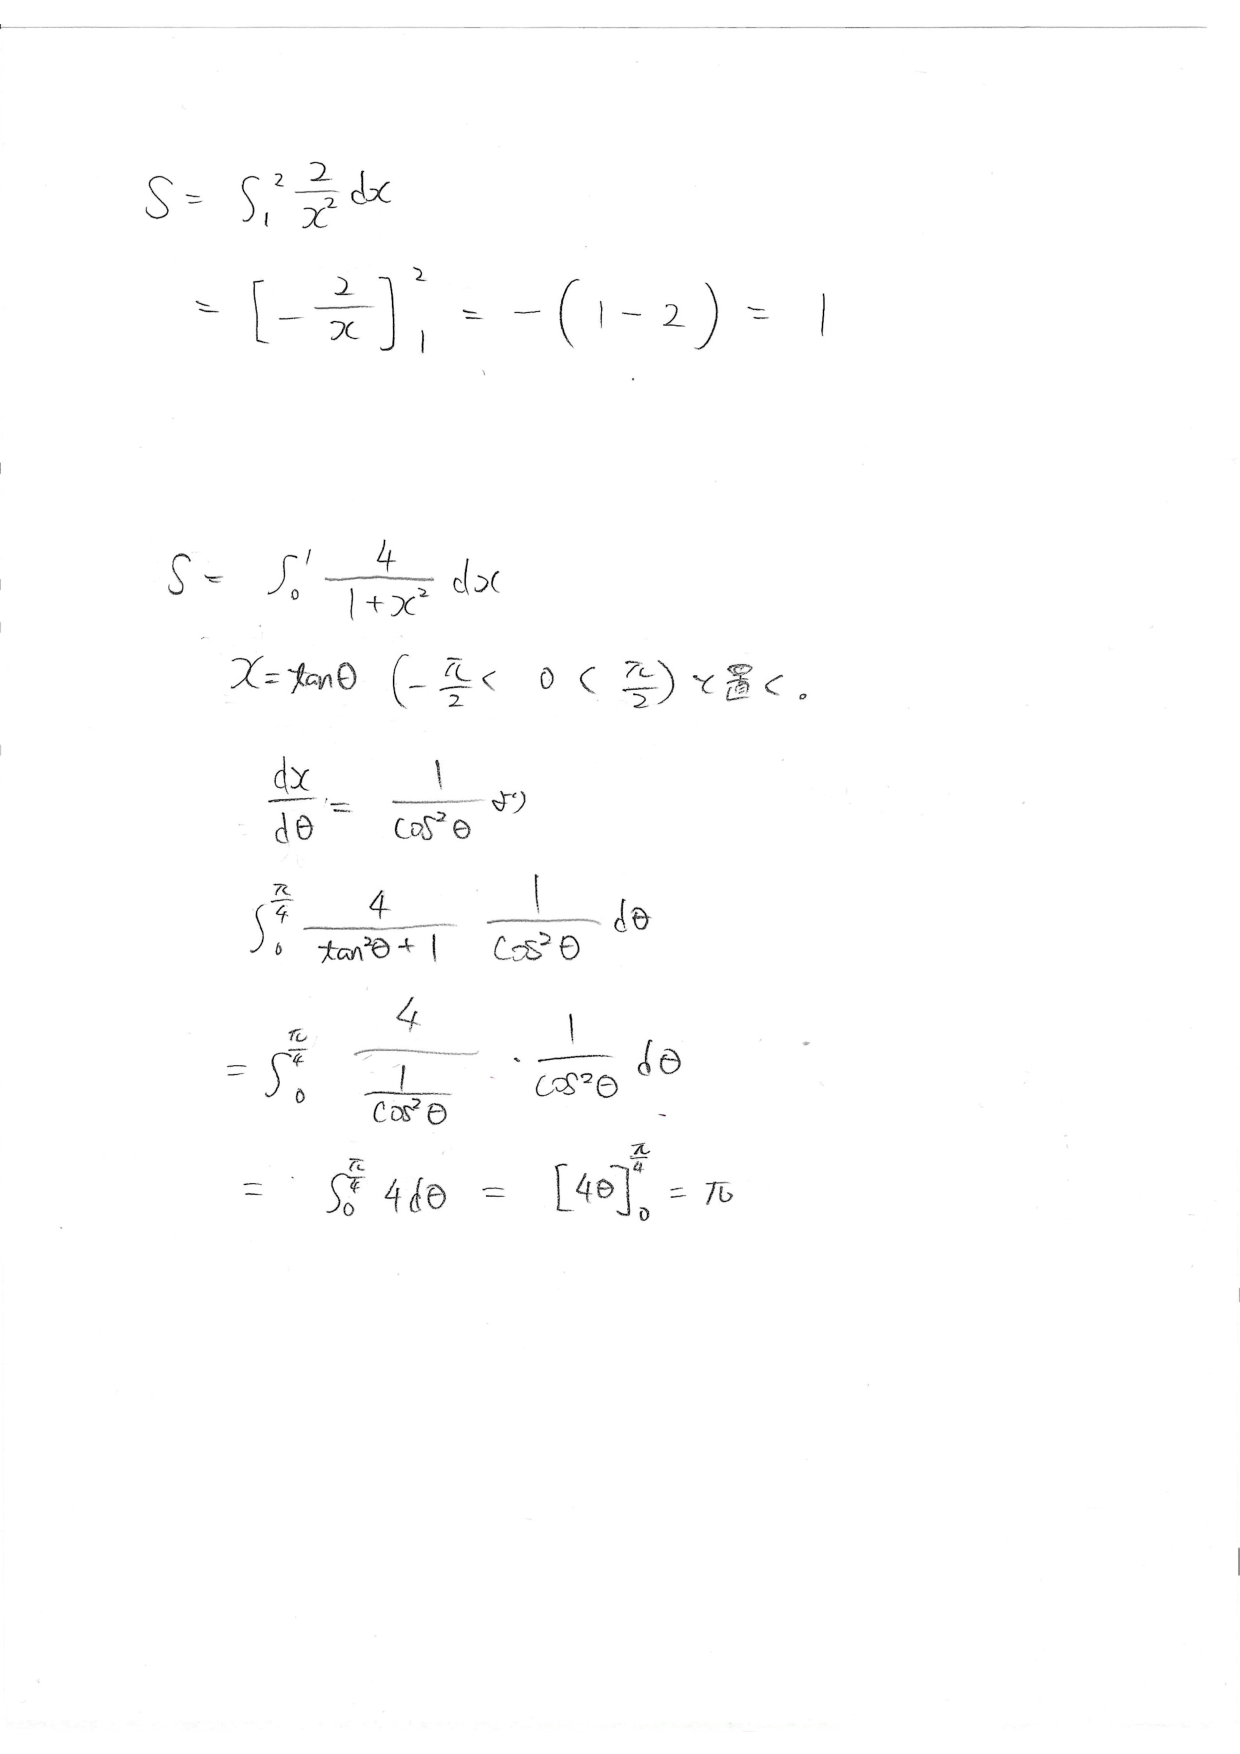
\includepdf[pages=-,noautoscale=true,scale=0.9,pagecommand={}]{futekesan.pdf}
定積分の結果は,$S=\int_{1}^{2}\frac{2}{x^2}dx$ = 1,$S=\int_{0}^{1}\frac{4}{1+x^2}dx$ = πとなった.
プログラムとの誤差を示すためそれぞれまとめる以下の表のようになった.
\begin{table}[H]
  \label{7}
  \begin{center}
  \caption{計算結果}
  \begin{tabular}{|l|l|l|l|}
  \hline
  定積分 & 台形公式 & シンプソン公式 & 手計算 \\ \hline
  $S=\int_{1}^{2}\frac{2}{x^2}dx$ &0.987529 &1 & 1 \\ \hline
  $S=\int_{0}^{1}\frac{4}{1+x^2}dx$&3.11157 & 3.141593 & π \\ \hline
\end{tabular}
\end{center}
\end{table}
\section{各公式において、分割数と結果の精度について考察}
結果は台形公式のほうが誤差があることになったが分割数を増やすとどうなるのか試してみる.
$S=\int_{1}^{2}\frac{2}{x^2}dx$の分割数nを10000にした場合.
\begin{verbatim}
genku@gen-mba output % ./"kadai4-1-1"
S=0.999875%
\end{verbatim}
$S=\int_{1}^{2}\frac{2}{x^2}dx$の分割数nを100000にした場合.
\begin{verbatim}
  genku@gen-mba output % ./"kadai4-1-1"
  S=0.999988% 
\end{verbatim}
$S=\int_{1}^{2}\frac{2}{x^2}dx$の分割数nを1000000にした場合.
\begin{verbatim}
  genku@gen-mba output % ./"kadai4-1-1"
  S=0.999999%  
\end{verbatim}
$S=\int_{1}^{2}\frac{2}{x^2}dx$の分割数nを10000000にした場合.
\begin{verbatim}
  genku@gen-mba output % ./"kadai4-1-1"
  S=1.000000%
\end{verbatim}
このようにシンプソン公式と比べて台形公式でより正確な値を出すには多くの分割数が必要だということがわかる.分割数が増えるたびに計算量が増えるので今回書いたプログラムではシンプソン公式のほうを使うのが効率がよいだろう.
\end{document}
